% This is text associated with the open textbook "Open Electromagnetics"
% See immediately below for author, date
% <License info goes here (boilerplate, not read by project compiler)>

%ORB TITLE Electric Field Intensity
%ORB AUTHOR 0        # S.W. Ellingson, Virginia Tech (ellingson@vt.edu)
%ORB DATE 20180731   # yyyymmdd
%ORB ABSTRACT 

\label{m0002_Electric_Field_Intensity} % <-- Must match name of this file and module directory name.  Don't mess with this!
\index{electric field intensity|(}
\index{field!electric|(}

\emph{Electric field intensity} is a vector field we assign the symbol ${\bf E}$ and has units of electrical potential per distance; 
in SI units, volts per meter (V/m).  
Before offering a formal definition, it is useful to consider the broader concept of the \emph{electric field}.
\index{field!electric}
\index{electric field|see{field, electric}}

Imagine that the universe is empty except for a single particle of positive charge.  
Next, imagine that a second positively-charged particle appears; the situation is now as shown in Figure~\ref{m0002_fTwoChargedParticles}.
Since like charges repel, the second particle will be repelled by the first particle and vice versa.
Specifically, the first particle is \emph{exerting force} on the second particle.
If the second particle is free to move, it will do so; this is an expression of kinetic energy.
\index{energy!kinetic}
\index{kinetic energy|see{energy, kinetic}}
If the second particle is somehow held in place, we say the second particle possesses an equal amount of potential energy.
\index{energy!potential}
\index{potential energy|see{energy, potential}} 
This potential energy is no less ``real,'' since we can convert it to kinetic energy simply by releasing the particle, thereby allowing it to move.
%
\begin{figure}[b!]
\begin{center}
\pdftooltip{{  % note double braces
\includegraphics[width=2in]{modules/m0002_fTwoChargedParticles.eps}
}}{Two circles with red plus signs in the middle to indicate their positive charge. They are some distance apart on the same horizontal axis indicated by a dashed line. An arrow labeled "F" is emanating from the rightmost particle and points to the right.}
\end{center}  
\centerline{\scriptsize 
\copyright~\hyperref[m0002_fTwoChargedParticles_Credit]{M.\ Goldammer} 
\href{https://creativecommons.org/licenses/by-sa/4.0/}{CC BY~SA 4.0} 
} 
\caption{
\label{m0002_fTwoChargedParticles}
A positively-charged particle experiences a repulsive force ${\bf F}$ in the presence of another particle which is also positively-charged.
% https://commons.wikimedia.org/wiki/File:M0002_fTwoChargedParticles.svg
}
\end{figure}

Now let us revisit the original one particle scenario.  In that scenario, we could make a map in which every position in space is assigned a vector that describes the force that a particle having a specified charge $q$ would experience if it were to appear there.  
The result looks something like Figure~\ref{m0002_fForceMap}. 
This map of force vectors is essentially a description of the electric field associated with the first particle.
%
\begin{figure}
\begin{center}
\pdftooltip{{  % note double braces
\includegraphics[width=2in]{modules/m0002_fForceMap.eps}
}}{A single circle with a red plus sign in it represents a positive charge. There are 8 arrows with a magnitude of "F" equidistantly spaced, emanating outward from the perimeter of the circle. Each of these arrows has a smaller arrow emanating from it.}
\end{center} 
\centerline{\scriptsize 
\copyright~\hyperref[m0002_fForceMap_Credit]{M.\ Goldammer} 
\href{https://creativecommons.org/licenses/by-sa/4.0/}{CC BY~SA 4.0} 
} 
\caption{
\label{m0002_fForceMap}
A map of the force that would be experienced by a second particle having a positive charge.  Here, the magnitude and direction of the force is indicated by the size and direction of the arrow.
% https://commons.wikimedia.org/wiki/File:M0002_fForceMap.svg
}
\end{figure}
 
There are many ways in which the electric field may be quantified. 
Electric field intensity ${\bf E}$ is simply one of these ways.  
We define ${\bf E}({\bf r})$ to be the force 
\index{force}
${\bf F}({\bf r})$ experienced by a test particle having charge $q$, divided by $q$; i.e.,  
%
\begin{equation}
{\bf E}({\bf r}) \triangleq \lim_{q \to 0} \frac{{\bf F}({\bf r})}{q}
\label{m0002_eEDef1}
\end{equation} 
%
Note that it is required for the charge to become vanishingly small (as indicated by taking the limit) in order for this definition to work.  
This is because the source of the electric field is charge, so the test particle contributes to the total electric field.  
To accurately measure the field of interest, the test charge must be small enough not to significantly perturb the field. 
This makes Equation~\ref{m0002_eEDef1} awkward from an engineering perspective, and we'll address that later in this section. 

According the definition of Equation~\ref{m0002_eEDef1}, the units of ${\bf E}$ are those of force divided by charge.  The SI units for force and charge are the newton (N) and coulomb (C) respectively, so ${\bf E}$ has units of N/C.  However, we typically express ${\bf E}$ in units of V/m, not N/C.  What's going on?  The short answer is that 1~V/m $=$ 1~N/C:
$$ 
\frac{\mbox{N}}{\mbox{C}} =
\frac{\mbox{N}\cdot\mbox{m}}{\mbox{C}\cdot\mbox{m}} =
\frac{\mbox{J}}{\mbox{C}\cdot\mbox{m}} =
\frac{\mbox{V}}{\mbox{m}}
$$
where we have used the fact that 1~N$\cdot$m $=$ 1~joule (J) of energy and 1~J/C $=$ 1~V. 

%ORB HIGHLIGHT
\begin{mdframed}[backgroundcolor=yellow!20,nobreak=true] 
Electric field intensity (${\bf E}$, N/C or V/m) 
\index{electric field intensity!definition}
is a vector field that quantifies the force experienced by a charged particle due to the influence of charge not associated with that particle. 
\end{mdframed}

The analysis of units doesn't do much to answer the question of why we should prefer to express ${\bf E}$ in V/m as opposed to N/C.
Let us now tackle that question.

Figure~\ref{m0002_fBatCap} shows a simple thought experiment that demonstrates the concept of electric field intensity in terms of an electric circuit.  
This circuit consists of a parallel-plate capacitor 
\index{capacitor!parallel plate}
in series with a 9~V battery.\footnote{It is not necessary to know anything about capacitors to get to the point, so no worries!}
The effect of the battery, connected as shown, is to force an accumulation of positive charge on the upper plate, and an accumulation of negative charge on the lower plate.  If we consider the path from the position labeled ``A,'' along the wire and through the battery to the position labeled ``B,'' the change in electric potential is $+9$~V.  It must also be true that the change in electric potential as we travel from B to A through the capacitor is $-9$~V, since the sum of voltages over any closed loop in a circuit is zero.  Said differently, the change in electric potential between the plates of the capacitor, starting from node A and ending at node B, is $+9$~V.  Now, note that the spacing between the plates in the capacitor is 1~mm.   
Thus, the rate of change of the potential between the plates is 9~V divided by 1~mm, which is 9000~V/m. 
This is literally the electric field intensity between the plates. 
That is, if one places a particle with an infinitesimally-small charge between the plates (point ``C''), and then measures the ratio of force to charge, one finds it is 9000~N/C pointing toward A.  We come to the following remarkable conclusion:
%
\begin{figure}
\begin{center}
\pdftooltip{{  % note double braces
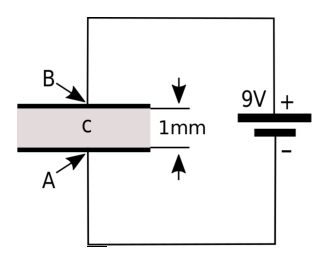
\includegraphics[width=2in]{modules/m0002_fBatCap.eps} 
% https://commons.wikimedia.org/wiki/File:M0002_fBatCap.svg
}}{Parallel plates joined in series with 9V battery. Upper plate labeled B, lower plate labeled A, and point between plates labeled C. Plates are 1 mm apart.}
\end{center}
\centerline{\scriptsize 
\copyright~\hyperref[m0002_fBatCap_Credit]{Y.\ Qin} 
\href{https://creativecommons.org/licenses/by/3.0/}{CC BY 3.0} 
} 
\caption{
\label{m0002_fBatCap}
A simple circuit used to describe the concept of electric field intensity. In this example, ${\bf E}$ at point C is 9000~V/m directed from B toward A. 
}
\end{figure}

%ORB HIGHLIGHT
\begin{mdframed}[backgroundcolor=yellow!20,nobreak=true] 
${\bf E}$ points in the direction in which electric potential is most rapidly decreasing, and the magnitude of ${\bf E}$ is the rate of change in electric potential with distance in this direction.  
\end{mdframed}

The reader may have noticed that we have defined the electric field in terms of what it \emph{does}.
We have have not directly addressed the question of what the electric field \emph{is}.  
This is the best we can do using classical physics, and
fortunately, this is completely adequate for the most engineering applications.
However, a deeper understanding is possible using quantum mechanics, 
\index{quantum mechanics}
where we find that the electric field and the magnetic field are in fact manifestations of the same fundamental force, aptly named the \emph{electromagnetic force}.
\index{electromagnetic force}
(In fact, the electromagnetic force is found to be one of just four fundamental forces, the others being \emph{gravity}, the \emph{strong nuclear force}, and the \emph{weak nuclear force}.)
Quantum mechanics also facilitates greater insight into the nature of electric charge and of the \emph{photon}, 
\index{photon}
which is the fundamental constituent of electromagnetic waves.  
For more information on this topic, an excellent starting point is the video ``Quantum Invariance \& The Origin of The Standard Model'' referenced at the end of this section.

%%%%%%%%%%%%%%%%%%%%%%%%%%

{\bf Additional Reading:}
\begin{itemize}
\item ``\href{https://en.wikipedia.org/wiki/Electric_field}{Electric field}'' on Wikipedia.
\item PBS Space Time video ``\href{https://youtu.be/V5kgruUjVBs}{Quantum Invariance} \& The Origin of The Standard Model,'' on YouTube.
\end{itemize}

\index{electric field intensity|)}
\index{field!electric|)}
